\documentclass[journal]{IEEEtran}

\usepackage{cite}
\usepackage{amsmath,amssymb,amsfonts}
\usepackage{algorithmic}
\usepackage{graphicx}
\usepackage{booktabs}
\usepackage{textcomp}
\usepackage{xcolor}
\usepackage{url}
\usepackage[hidelinks]{hyperref}

\hyphenation{op-tical net-works semi-conduc-tor}

\begin{document}

\title{Reducing False Negatives in IoT Malware Detection: A Comparative Study of Balancing Strategies on Three Real NIDS Datasets}

\author{Carlos~A.~C.~Tojeiro,\IEEEauthorrefmark{1}
        Thiago~J.~Lucas,\IEEEauthorrefmark{1}
        and~Kelton~A.~P.~da~Costa,~\IEEEmembership{Senior Member,~IEEE}\IEEEauthorrefmark{1}%
\thanks{Carlos A. C. Tojeiro, Thiago J. Lucas, and Kelton A. P. da Costa are with the Department of Computing, S\~ao Paulo State University (UNESP), Bauru, Brazil (e-mail: carlos.tojeiro@unesp.br; t.lucas@unesp.br; kelton.costa@unesp.br).}}

\markboth{IEEE Internet of Things Journal,~Vol.~XX, No.~XX, Month~Year}%
{Tojeiro \MakeLowercase{\textit{et al.}}: Reducing False Negatives in IoT Malware Detection}

\maketitle

\begin{abstract}
This paper studies how the class imbalance of real network traffic degrades machine-learning-based intrusion detection systems (IDSs). When attacks are rare relative to benign flows, detectors become biased toward the majority class and silently miss malware---a false negative (FN), the costliest error in security. Generative adversarial networks (GANs) are increasingly used to oversample minority attack classes, but most studies report aggregate accuracy or F1-score and rarely quantify the impact of the balancing strategy on the false-negative count or isolate it from the classifier. We compare six balancing strategies---none, SMOTETomek, a vanilla GAN, WGAN-GP, cWGAN-GP, and CTGAN---under a strictly controlled, identical protocol reproduced on three real public datasets (CICIDS2017, UNSW-NB15, and IoT-23) and four classifiers (MLP, XGBoost, Random Forest, and LSTM), sharing the same workload (40{,}000 flows, 82\% benign / 18\% attack), split, feature-selection step, and test set, so that any difference is attributable only to the balancing method. The benefit is strongly classifier-dependent: the LSTM is the most improved, cutting false negatives by 83.1\% on CICIDS2017, 81.5\% on UNSW-NB15, and 40.6\% on IoT-23; tree ensembles gain only marginally; and MLP gains are inconsistent. No strategy dominates, and the vanilla GAN is the most expensive, making WGAN-GP the cheapest generator.
\end{abstract}

\begin{IEEEkeywords}
Internet of Things, intrusion detection, botnet, class imbalance, oversampling, generative adversarial networks, CTGAN, WGAN-GP, false negatives, CICIDS2017, UNSW-NB15, IoT-23.
\end{IEEEkeywords}

\section{Introduction}
\IEEEPARstart{T}{he} Internet of Things (IoT) connects billions of resource-constrained devices whose default posture is often insecure, making botnets such as Mirai, Torii, and Hajime a persistent and growing threat~\cite{frustaci2018iotsecurity,zou2016wireless}. Network-based intrusion detection systems (NIDS) are a first line of defense, and machine learning (ML) has become the dominant paradigm for detecting malicious traffic at the flow level~\cite{khraisat2019survey,ring2019survey}. However, ML-based NIDS are confronted with a fundamental obstacle: real network traffic is severely class-imbalanced. In the IoT-23 dataset~\cite{garcia2020iot23}, for example, benign flows vastly outnumber malicious ones in most captures, and even within malicious traffic the relevant attack families are minority classes.

Class imbalance biases classifiers toward the majority class. The most dangerous consequence is not a slightly lower accuracy but a higher number of \emph{false negatives}---malware flows that the detector classifies as benign and therefore allows into the network. In a security context, the cost of a missed attack (compromised device, lateral movement, botnet recruitment) is orders of magnitude higher than the cost of a false alarm that an operator can inspect~\cite{he2023cwvaegan}. Yet the overwhelming majority of papers in the NIDS literature optimize and report aggregate metrics---accuracy, precision, recall, F1-score---and either do not report the confusion-matrix counts or do not isolate the effect of the balancing method from that of the classifier architecture.

Among the techniques proposed to mitigate imbalance, oversampling has proven effective. Classic interpolation methods such as SMOTE~\cite{chawla2002smote} and its variants (SMOTE-ENN, SMOTETomek~\cite{batista2004smoteenn}, ADASYN~\cite{he2008adasyn}) create synthetic minority samples by interpolating between neighbors in feature space. Generative adversarial networks (GANs)~\cite{goodfellow2014gan} and their refinements---WGAN~\cite{arjovsky2017wgan}, WGAN-GP~\cite{gulrajani2017wgangp}, conditional GANs~\cite{mirza2014cgan}, and the conditional tabular GAN (CTGAN)~\cite{xu2019ctgan}---learn the underlying data distribution and are increasingly used to synthesize minority attack samples~\cite{park2023ainids,habibi2023ctgan,yao2025cwgangp,rahman2024syngan,engelmann2021cwgan}.

Several recent works report impressive results with GAN-based oversampling in NIDS. A-NIDS~\cite{zha2025anids} combines clustering with stacked CTGAN to handle data drift and catastrophic forgetting. He et al.~\cite{he2023cwvaegan} propose CWVAEGAN-1DCNN, a conditional Wasserstein variational autoencoder with GAN that generates minority samples and achieves high recall for rare attack classes. Soflaei et al.~\cite{soflaei2024dualctgan} use CTGAN-balanced data with a dual-ensemble of weak classifiers, reaching 98\% binary classification accuracy on UNSW-NB15. CE-GAN~\cite{yang2025cegan} couples a conditional GAN with an aggregation encoder-decoder and a composite loss, improving minority-class metrics on NSL-KDD and UNSW-NB15. SYN-GAN~\cite{rahman2024syngan} trains NIDS models entirely on GAN-synthesized traffic (UNSW-NB15, NSL-KDD, and BoT-IoT). However, these studies differ in datasets, features, classifiers, and evaluation protocols, which makes their results difficult to compare and prevents any conclusion about which generator family is most effective at reducing false negatives on a given IDS benchmark.

In this paper we perform a strictly controlled comparison of six balancing strategies on a fixed binary detection protocol that is reproduced, unchanged, on \emph{three real public datasets}: CICIDS2017~\cite{sharafaldin2018cicids}, UNSW-NB15~\cite{moustafa2015unsw}, and the IoT-23 dataset~\cite{garcia2020iot23} collected by the Stratosphere Laboratory, and across \emph{four classifiers}: MLP, XGBoost~\cite{chen2016xgboost}, Random Forest~\cite{breiman2001rf}, and LSTM~\cite{hochreiter1997lstm}. Every dataset is reduced to an identical workload of 40{,}000 flows (82\% benign / 18\% attack), split 70/30 with the same seed, and preprocessed with the same \texttt{StandardScaler} $+$ \texttt{SelectPercentile} step; the only variable that changes across experiments is the balancing strategy added between preprocessing and classification. All results are reported on the same per-dataset test set, and the analysis emphasizes confusion-matrix counts rather than aggregate metrics alone, with a selection rule (Section~\ref{sec:method}) that avoids rewarding a strategy that reduces FNs at the price of a collapsed F1-score.

Our main findings are as follows.
\begin{itemize}
\item The balancing benefit is concentrated in the deep sequential classifier. The LSTM is the model most degraded by imbalance---F1 of 0.33, 0.71, and 0.62 in the three unbalanced baselines---and the one most improved by resampling: FNs are cut by 83.1\% on CICIDS2017 (1{,}716$\rightarrow$290, cWGAN-GP), 81.5\% on UNSW-NB15 (845$\rightarrow$156, SMOTETomek), and 40.6\% on IoT-23 (1{,}169$\rightarrow$694, WGAN-GP).
\item Tree ensembles are largely unaffected: XGBoost misses only four attacks on CICIDS2017 without any balancing, and oversampling adds at most 16--17\% FN reduction (UNSW-NB15) for them. This is consistent with the known robustness of boosting and bagging to moderate imbalance.
\item The MLP shows no reliable benefit. Its CICIDS2017 baseline (37 FNs) is \emph{never} improved by balancing (best balanced configuration yields 60), the gain on UNSW-NB15 is marginal, and the result on IoT-23 is neutral---evidence that in easy, near-separable problems synthetic oversampling can only add label noise.
\item No single strategy dominates. Classic SMOTETomek and the Wasserstein-based generative methods (WGAN-GP, cWGAN-GP) alternate as the best configuration across datasets and models, while CTGAN remains a consistently strong option. Headlines that crown a single generator family overstate the evidence.
\item The five findings above are \emph{invisible} when only accuracy or F1 is reported; a confusion-matrix-oriented, per-classifier protocol is therefore essential to evaluate balancing strategies in security contexts.
\end{itemize}

The remainder of this paper is organized as follows. Section~\ref{sec:bg} reviews GAN families and balancing strategies for NIDS. Section~\ref{sec:method} details the three datasets, the experimental protocol, and the six balancing pipelines. Section~\ref{sec:results} presents and discusses the cross-dataset results. Section~\ref{sec:conclusion} concludes and outlines future work.

\section{Background and Related Work}
\label{sec:bg}

\subsection{Generative Adversarial Networks and Their Variants}
\label{sec:ganfamily}
A GAN~\cite{goodfellow2014gan} trains two networks in a zero-sum game: a generator $G$ maps latent noise $\mathbf{z} \sim p_z$ to synthetic samples, and a discriminator $D$ distinguishes real from generated samples. Training minimizes a Jensen-Shannon (JS) divergence proxy, which is known to suffer from vanishing gradients and mode collapse~\cite{arjovsky2017wgan}. The Wasserstein GAN~\cite{arjovsky2017wgan} replaces the JS objective with the Wasserstein-1 distance, yielding a critic whose gradients remain informative even when the distributions do not overlap. WGAN-GP~\cite{gulrajani2017wgangp} enforces the Lipschitz constraint with a gradient penalty, greatly improving training stability. Conditional GANs~\cite{mirza2014cgan} condition both networks on auxiliary information (e.g., class labels), enabling controlled generation of samples from a specific class---a property that is directly useful for oversampling the minority class.

For tabular data, Xu et al.~\cite{xu2019ctgan} proposed CTGAN, which addresses two fundamental problems of GANs on tabular data: (i) continuous columns rarely follow a Gaussian distribution, which they handle with mode-specific normalization based on a Gaussian mixture model (GMM); and (ii) the generator cannot easily sample from all the discrete modes of a categorical column, which they address with conditional vectors and training-by-sampling, together with a pac discriminator (pacs$=$10) to mitigate mode collapse. These design choices make CTGAN particularly well suited to network-flow data, whose continuous features (durations, packet and byte statistics) are typically multimodal.

\subsection{Oversampling Strategies for Network Intrusion Detection}
Resampling is the most widely used countermeasure against imbalance in NIDS. SMOTE~\cite{chawla2002smote} interpolates between minority-class neighbors; SMOTETomek and SMOTE-ENN~\cite{batista2004smoteenn} combine SMOTE with cleaning rules (Tomek links or edited nearest neighbors) to remove noisy and overlapping samples; ADASYN~\cite{he2008adasyn} adapts the number of generated samples to the local density of the minority class. These methods are simple and fast, but their linear interpolation can generate unrealistic samples when the minority class is multimodal or overlaps the majority class, and recent large-scale studies still report inconsistent gains in IoT settings~\cite{talukder2024mlstl,albasheer2024jaya,talukder2024jbigdata}.

GAN-based oversampling learns the data distribution instead of interpolating locally. Engelmann and Lessmann~\cite{engelmann2021cwgan} showed that conditional Wasserstein GANs are competitive with classic oversampling for tabular credit data, and this line of work was extended to NIDS by numerous authors, including GAN augmentation for imaging-based intrusion detection~\cite{andresini2021ganaug}. Zheng et al.~\cite{zheng2020cwgangp} introduced CWGAN-GP for imbalanced classification, and Yao and Zhao~\cite{yao2025cwgangp} applied CWGAN-GP oversampling to intrusion detection, reporting better classification than traditional oversampling algorithms on two benchmark datasets. Ding et al.~\cite{ding2024tmgggan} proposed TMG-GAN, a GAN-based imbalanced learning method for NIDS published in IEEE TIFS. Swadi and Al-Mashhadi~\cite{swadi2025wcg} used Wasserstein conditional GANs for class balancing in intrusion detection datasets. WCGAN-GP has also been combined with XGBoost classifiers in flow-based IDS~\cite{vo2024apelid}, and GAN-augmented anomaly detection has been applied to IoT malware detection~\cite{moti2021ganiot}.

CTGAN, in particular, has attracted growing attention in the NIDS literature. Habibi et al.~\cite{habibi2023ctgan} modeled imbalanced tabular IoT data with CTGAN and machine learning to improve IoT botnet attack detection. Alabsi et al.~\cite{alabsi2023ctgan} built a CTGAN-based IDS for DDoS and DoS attacks. A-NIDS~\cite{zha2025anids} uses stacked CTGAN for continual-learning-aware detection. Soflaei et al.~\cite{soflaei2024dualctgan} combined CTGAN-balanced data with weak classifiers and an XGBoost meta-classifier, reporting 98\% binary accuracy on UNSW-NB15. CE-GAN~\cite{yang2025cegan} augments rare samples with a conditional aggregation encoder-decoder and a composite loss. Other generative approaches include CWVAEGAN-1DCNN~\cite{he2023cwvaegan}, which uses a variational Gaussian mixture decomposition before generation, MCGAN~\cite{babu2023mcgan}, DAE-GAN~\cite{li2022daegan}, and SYN-GAN~\cite{rahman2024syngan}, which targets IoT security on IoT-23.

\subsection{Generative Data for IoT Security and Datasets}
The choice of benchmark strongly influences reported performance. Common IoT and general-purpose NIDS datasets include N-BaIoT~\cite{meidan2018nbahot}, Bot-IoT~\cite{koroniotis2019botiot}, Edge-IIoTset~\cite{ferrag2022edgeiiotset}, UNSW-NB15~\cite{moustafa2015unsw}, NSL-KDD~\cite{tavallaee2009nslkdd}, and the recent surveys in~\cite{ring2019survey,khraisat2019survey}. The IoT-23 dataset~\cite{garcia2020iot23} was captured in the Stratosphere Laboratory with 20 malware captures (Mirai, Torii, Hajime, Gagfyt, and others) and three benign IoT device captures (Philips HUE, Amazon Echo, Somfy doorlock). It is one of the most realistic and recently collected labeled IoT datasets, and it has been used in recent ML-based detection challenges~\cite{moti2021ganiot}. Nevertheless, most IoT-23 studies either use flow-level features from the full multi-gigabyte capture or restrict themselves to a single scenario, and few report the detailed confusion matrix that would reveal the false-negative count. Anomaly-detection baselines such as Kitsune~\cite{mirsky2018kitsune}, flow-level traffic generation with GANs~\cite{ring2019flowgan}, and hybrid deep models that analyze imbalance and robustness jointly~\cite{wang2023hybrid} complement the generative-oversampling literature. Moti et al.~\cite{moti2021ganiot} used GANs to detect unseen IoT malware, and Rahman et al.~\cite{rahman2024syngan} trained NIDS models on fully synthetic GAN data, but neither performs a head-to-head comparison of generator families under a fixed pipeline.

\subsection{Gaps and Positioning}
Three gaps motivate our work. First, existing studies compare generative oversampling methods against each other or against SMOTE under \emph{different} classifiers, datasets, or feature sets, making the marginal contribution of the generator impossible to isolate. Second, almost no study reports false negatives as a first-class metric, even though it is the security-critical error. Third, there is no controlled benchmark of classic resampling (SMOTETomek) against generative baselines (vanilla GAN, WGAN-GP, cWGAN-GP, CTGAN) reproduced identically on multiple real datasets and classifiers. Our contribution addresses these gaps with a strictly controlled protocol on three real datasets, described next. Beyond the empirical comparison, we make a methodological contribution that is, to our knowledge, absent from the NIDS oversampling literature: we report the \emph{full confusion matrix} (including the security-critical FN count) for every balancing strategy--classifier--dataset configuration and we frame the paper around ``\emph{what each strategy {\color{black}does not} fix}'' rather than around best-rows. This honest framing is what allows us to conclude that no single generator family dominates and that balancing benefits are strongly classifier- and dataset-dependent---conclusions that aggregate-metric-only papers cannot sustain.

\section{Methodology}
\label{sec:method}

\subsection{Datasets and Preprocessing}
We use three public, real, labeled network-traffic datasets. \textbf{CICIDS2017}~\cite{sharafaldin2018cicids} is a five-day enterprise-network capture (Monday--Friday) with modern attacks performed at controlled times and processed by CICFlowMeter into flow features; its eight daily files are concatenated. \textbf{UNSW-NB15}~\cite{moustafa2015unsw} was generated in the UNSW Canberra Cyber Range with the IXIA PerfectStorm tool, combining normal traffic and modern attacks (Fuzzing, Backdoors, DoS, Exploits, Reconnaissance, Shellcode, Worms) characterized by 45 flow features; we use the official training file. \textbf{IoT-23}~\cite{garcia2020iot23} was captured by the Stratosphere Laboratory and contains benign flows from three real smart-home devices (Philips HUE, Amazon Echo, Somfy doorlock) and malicious flows from multiple botnets (Mirai, Torii, Hajime, Gagfyt, and others); we use a preprocessed mirror of the Zeek \texttt{conn.log} records ($6.05$M flows, 21 columns), kept binary as benign vs.\ malicious.

To make the three datasets directly comparable, each is reduced to an identical workload through stratified sampling. From each full dataset we draw a stratified sample of exactly \textbf{40{,}000 flows with 82\% benign (32{,}800) and 18\% attack (7{,}200)} using a fixed seed (42), which mirrors the imbalance regime of real IoT traffic in which attacks are the minority. The sample is split 70/30 stratified: \textbf{28{,}000 training} flows (22{,}960 benign, 5{,}040 attack) and \textbf{12{,}000 test} flows (9{,}840 benign, 2{,}160 attack), guaranteeing that the test set is identical across all six balancing strategies for a given dataset. Numeric flow features are standardized with \texttt{StandardScaler}, and feature selection is performed with \texttt{SelectPercentile} (ANOVA $f$-classif, 60\%), fitted on the training split only and reused on the test split to avoid any information leak, using scikit-learn~\cite{pedregosa2011sklearn}. For IoT-23 the features are the Zeek \texttt{conn.log} fields (durations, bytes, packets, ports, \texttt{missed\_bytes}); for UNSW-NB15 and CICIDS2017 they are the flow-level features of the respective formats. The pipeline is summarized in Fig.~\ref{fig:pipeline}.

\begin{figure}[!t]
\centering
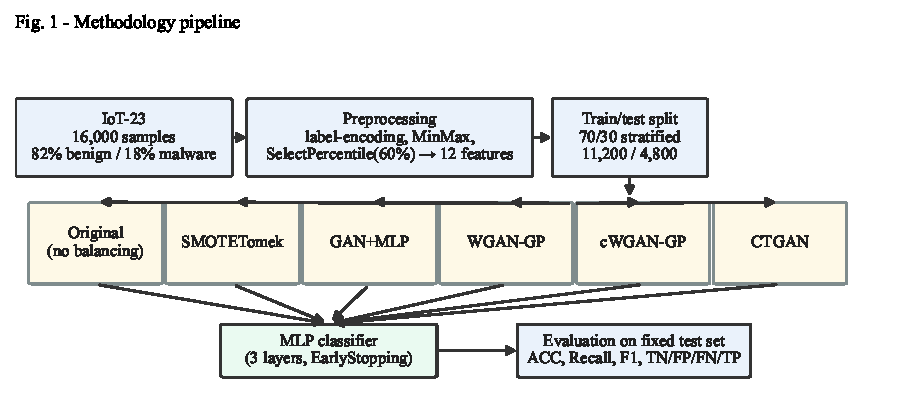
\includegraphics[width=\columnwidth]{figures/fig1_pipeline.pdf}
\caption{Experimental pipeline. For each of the three real datasets (CICIDS2017, UNSW-NB15, IoT-23), 40{,}000 flows (82\% benign / 18\% attack) are preprocessed (\texttt{StandardScaler}, \texttt{SelectPercentile} 60\%) and split 70/30 stratified (seed 42). The training set (28{,}000 flows) is balanced by one of six strategies, each classifier is trained, and evaluation is performed on the fixed test set (12{,}000 flows, 9{,}840 benign / 2{,}160 attack).}
\label{fig:pipeline}
\end{figure}

\subsection{Balancing Strategies}
Six strategies are applied to the training split before classification. Fig.~\ref{fig:pipeline} summarizes the flow. Each generative strategy produces exactly 17{,}920 synthetic attack-flows, rebalancing the minority class to parity (5{,}040 $\rightarrow$ 22{,}960), so that the augmented training set contains 45{,}920 flows.

\subsubsection{No Balancing (Baseline)}
The original imbalanced training set (82\% benign) is used directly. This baseline quantifies the bias introduced by imbalance and the maximum false-negative count each classifier can produce, and is the reference against which all reductions are measured.

\subsubsection{SMOTETomek}
SMOTETomek~\cite{batista2004smoteenn} first applies SMOTE ($k{=}5$) to synthesize new malicious samples, then removes Tomek-link pairs to clean class boundaries. It represents the state of the art among classic resampling hybrids and serves as the non-generative reference strategy.

\subsubsection{Vanilla GAN}
A standard GAN~\cite{goodfellow2014gan} is trained on the minority (attack) samples only. The generator maps 32-dimensional Gaussian noise through three dense layers (64, 128, 256) with batch normalization~\cite{ioffe2015batchnorm}, ReLU, and a \texttt{tanh} output; the discriminator uses two dense layers (256, 128) with dropout (0.3) and a sigmoid output. Training uses binary cross-entropy with Adam~\cite{kingma2015adam} ($2\times10^{-4}$, $\beta_1{=}0.5$), batch size 64, 300 epochs. After training, 17{,}920 samples are drawn from the generator.

\subsubsection{WGAN-GP}
WGAN-GP~\cite{gulrajani2017wgangp} replaces the discriminator with a critic that outputs a real value (no sigmoid), trained to minimize the Wasserstein distance with gradient-penalty coefficient $\lambda{=}10$ and five critic updates per generator update ($n_{\mathrm{critic}}{=}5$). Architectures and optimizer settings are otherwise identical to the vanilla GAN. This variant isolates the contribution of the Wasserstein loss alone (no class conditioning).

\subsubsection{Conditional WGAN-GP (cWGAN-GP)}
cWGAN-GP extends WGAN-GP with class conditioning~\cite{mirza2014cgan,yao2025cwgangp}: both the generator and the critic receive the class label through an embedding layer (2 classes $\rightarrow$ 16 dimensions) concatenated to the input. The model is trained on the complete training set, so that the generator learns both modes, and generation is performed conditioned on the malicious class, producing 17{,}920 samples that respect the conditional distribution.

\subsubsection{CTGAN}
CTGAN~\cite{xu2019ctgan} is trained on the complete training set using its default mode-specific normalization: each continuous feature is decomposed with a variational Gaussian mixture model, and categorical features are encoded with one-hot vectors plus conditional sampling via training-by-sampling. The network uses the standard CTGAN architecture (2 hidden layers of 256 units) with a pac discriminator ($\mathrm{pacs}{=}10$), batch size 200, and 300 epochs. A total of 17{,}920 samples are then generated conditioned on the malicious class.

\subsection{Classifiers}
Four classifiers are trained on each (possibly augmented) training set and evaluated on the same test set.
\begin{itemize}
\item \textbf{MLP}: two hidden dense layers (128 and 64 neurons, ReLU) with dropout (0.3), a sigmoid output, Adam ($10^{-3}$), binary cross-entropy, batch size 64, up to 60 epochs with early stopping (patience 6) on validation loss.
\item \textbf{XGBoost}~\cite{chen2016xgboost}: 300 trees, learning rate 0.05, maximum depth 6, subsample and column subsample 0.8, histogram-based training.
\item \textbf{Random Forest}~\cite{breiman2001rf}: 300 trees.
\item \textbf{LSTM}~\cite{hochreiter1997lstm}: two stacked LSTM layers (64 and 32 units) with dropout (0.3), a sigmoid output, Adam ($10^{-3}$), binary cross-entropy, batch size 64, up to 60 epochs with early stopping (patience 6). Each flow is presented as a sequence of $n$ timesteps where $n$ is the number of selected features, one feature per timestep.
\end{itemize}

Table~\ref{tab:hparams} summarizes the hyperparameters; a fixed random seed (42) is used throughout.

\begin{table}[!t]
\caption{Hyperparameters of the Balancing Pipelines and Classifiers}
\label{tab:hparams}
\begin{center}
\begin{tabular}{@{}ll@{}}
\toprule
\textbf{Component} & \textbf{Setting} \\
\midrule
Workload & 40{,}000 flows (82\%/18\%), stratified, seed 42 \\
Split & 70/30 stratified, seed 42 (train 28{,}000 / test 12{,}000) \\
Preprocessing & \texttt{StandardScaler} + \texttt{SelectPercentile} (60\%) \\
Synthetic target & 17{,}920 samples (minority 5{,}040 $\rightarrow$ 22{,}960) \\
SMOTETomek & SMOTE $k{=}5$ + Tomek links \\
GAN & noise 32; G: 64--128--256 + BN + tanh; \\
 & D: 256--128 + Dropout(0.3) + sigmoid \\
 & 300 epochs, batch 64, Adam $2\times10^{-4}$, $\beta_1{=}0.5$ \\
WGAN-GP & $\lambda{=}10$, $n_{\mathrm{critic}}{=}5$, critic linear \\
cWGAN-GP & + label embedding (2$\rightarrow$16) on G and D \\
CTGAN & 300 epochs, batch 200, $\mathrm{pacs}{=}10$, GMM normalization \\
MLP & 128--64 ReLU + Dropout(0.3), sigmoid, Adam $10^{-3}$ \\
 & batch 64, 60 epochs, early stop patience 6 \\
XGBoost & 300 trees, lr 0.05, depth 6, subsample/colsample 0.8 \\
Random Forest & 300 trees \\
LSTM & LSTM(64, return seq) + LSTM(32), Dropout(0.3) \\
 & Adam $10^{-3}$, batch 64, 60 epochs, patience 6 \\
 & input reshaped to ($n_{\mathrm{features}}$, 1) \\
\bottomrule
\end{tabular}
\end{center}
\end{table}

\subsection{Evaluation Metrics}
Let TN, FP, FN, and TP be the counts of true negatives, false positives, false negatives, and true positives on the fixed test set of a given dataset. We report accuracy (ACC), precision (P), recall (R), and F1-score:
\begin{align}
\mathrm{ACC} &= \frac{TP+TN}{TP+TN+FP+FN}, \label{eq:acc}\\
\mathrm{P} &= \frac{TP}{TP+FP}, \qquad \mathrm{R} = \frac{TP}{TP+FN}, \label{eq:pr}\\
\mathrm{F1} &= \frac{2\cdot \mathrm{P}\cdot \mathrm{R}}{\mathrm{P}+\mathrm{R}}. \label{eq:f1}
\end{align}
In addition, we analyze FN and FP counts explicitly, since in security applications a false negative (missed malware) is the most costly error. Because a naive ``minimum-FN'' rule can select a scenario that reduces FNs at the price of a collapsed F1-score (e.g., a generator with high recall but very low precision), we adopt an explicit selection rule for the ``best balanced configuration'' reported in Table~\ref{tab:cross}: \emph{among the five balanced scenarios, choose the one with the smallest FN whose F1-score stays within 0.05 of the best F1-score achieved by any balanced scenario for that model and dataset}. This rule is described a-priori, avoids cherry-picking, and is applied identically to all results. To quantify the sampling uncertainty around the point estimates, we also compute 95\% confidence intervals by Monte Carlo propagation of the binomial test counts: 200{,}000 draws of $TP\sim\mathrm{Binomial}(TP+FN,\hat{R})$ and $FP\sim\mathrm{Binomial}(TN+FP,1-\widehat{\mathrm{TNR}})$ yield distributions of FN, precision, recall, and F1, summarized by their 2.5th and 97.5th percentiles. These intervals quantify the finite-sample binomial uncertainty on the fixed test set and are not adjusted for the multiple comparisons across the 24 model-dataset scenarios; they should therefore be read per row rather than as family-wise tests. The complete intervals for all 72 configurations and the tolerance-sensitivity analysis are provided as supplementary material (Supplementary Tables S1 and S2).

\section{Results and Discussion}
\label{sec:results}

\subsection{Cross-Dataset Detection Performance}
Table~\ref{tab:cross} reports, for each of the three real datasets and four classifiers: the false-negative count of the imbalanced baseline, the false-negative count of the best balanced configuration under the rule of Section~\ref{sec:method}, the selected balancing strategy, its false-positive count, and the resulting FN change. Twelve configurations in total share the same workload, split, preprocessing, and test set; the only difference across rows is the dataset and the classifier.

\begin{table*}[!t]
\caption{Cross-Dataset Validation on Three Real Datasets: False-Negative Reduction at the Best Balancing Strategy (FN counts on the fixed 12{,}000-flow test set)}
\label{tab:cross}
\centering
\footnotesize
\setlength{\tabcolsep}{6pt}
\begin{tabular}{@{}lcccclll@{}}
\toprule
\textbf{Dataset} & \textbf{Clf} & \textbf{FN (base)} & \textbf{FN (best)} & \textbf{Strategy} & \textbf{FP (best)} & \textbf{$\Delta$FN} & \textbf{F1 (best)} \\
\midrule
CICIDS2017 & MLP & 37 & 60 & GAN & 180 & $+62.2\%$ & 0.9459 \\
CICIDS2017 & XGBoost & 4 & 4 & SMOTETomek & 7 & $0\%$ & 0.9975 \\
CICIDS2017 & R. Forest & 14 & 7 & SMOTETomek & 3 & $-50.0\%$ & 0.9977 \\
CICIDS2017 & LSTM & 1{,}716 & 290 & cWGAN-GP & 553 & $-83.1\%$ & 0.8161 \\
UNSW-NB15 & MLP & 421 & 404 & GAN & 139 & $-4.0\%$ & 0.8661 \\
UNSW-NB15 & XGBoost & 303 & 253 & SMOTETomek & 224 & $-16.5\%$ & 0.8888 \\
UNSW-NB15 & R. Forest & 298 & 248 & SMOTETomek & 211 & $-16.8\%$ & 0.8928 \\
UNSW-NB15 & LSTM & 845 & 156 & SMOTETomek & 1{,}343 & $-81.5\%$ & 0.7278 \\
IoT-23 & MLP & 636 & 638 & WGAN-GP & 25 & $\approx0\%$ & 0.8211 \\
IoT-23 & XGBoost & 273 & 272 & SMOTETomek & 25 & $\approx0\%$ & 0.9271 \\
IoT-23 & R. Forest & 269 & 267 & cWGAN-GP & 134 & $-0.7\%$ & 0.9042 \\
IoT-23 & LSTM & 1{,}169 & 694 & WGAN-GP & 171 & $-40.6\%$ & 0.7722 \\
\bottomrule
\multicolumn{8}{@{}l}{{\footnotesize \textit{Note:} GAN denotes the vanilla GAN of Section~\ref{sec:method}; the remaining strategy names follow Table~\ref{tab:hparams}.}}\\
\end{tabular}
\end{table*}

Three findings emerge from Table~\ref{tab:cross}. First, the benefit of balancing is highly classifier-dependent and is concentrated in the deep sequential model. The LSTM is the classifier most degraded by imbalance---its unbalanced baselines carry F1-scores of only 0.33 (CICIDS2017), 0.71 (UNSW-NB15), and 0.62 (IoT-23)---and is also the one that benefits the most from resampling: FNs drop by 83.1\%, 81.5\%, and 40.6\% on the three datasets ($1{,}716\rightarrow290$, $845\rightarrow156$, and $1{,}169\rightarrow694$, respectively), with the F1-score rising to 0.82, 0.73, and 0.77. Fig.~\ref{fig:confusion} shows the confusion matrices of the LSTM in the unbalanced baseline and in the best balanced configuration for each dataset. The improvement is not an artifact of the selection rule: the 95\% Monte Carlo binomial confidence intervals of the balanced F1-scores---0.82~[0.80,~0.83], 0.73~[0.72,~0.74], and 0.77~[0.76,~0.79]---do not overlap those of the unbalanced baselines---0.33~[0.30,~0.35], 0.71~[0.69,~0.72], and 0.62~[0.60,~0.63]. The reduction is concentrated in the false-negative cell (actual attack, predicted benign): the LSTM's attack recall rises from 0.21 to 0.87 on CICIDS2017, from 0.61 to 0.93 on UNSW-NB15, and from 0.46 to 0.68 on IoT-23, while false positives stay bounded on CICIDS2017 and IoT-23 (553 and 171, respectively) but rise substantially on UNSW-NB15 (1{,}343, about 13.6\% of the benign test flows). This is the precision cost of the SMOTETomek row chosen there; under the asymmetric cost structure of security (FN cost $\gg$ FP cost) the FN reduction still dominates, and the F1-guard prevents the full precision collapse that a naive min-FN rule would cause---but the exact trade-off depends on the deployment thresholds, which is precisely why we report both counts explicitly. The particularly strong effect on the LSTM is consistent with its larger capacity and with the fact that it is the classifier most degraded by imbalance: once resampling keeps the recurrent layers from collapsing onto the majority class, the model recovers most of the minority signal. Because the input is a pseudo-sequence (one standardized feature per timestep, in column order, Section~\ref{sec:method}), we do not attribute the gain to a genuine temporal structure of the flows; whether order-aware sequential inputs (e.g., per-connection Zeek event sequences) amplify the benefit is left to future work.

\begin{figure*}[!t]
\centering
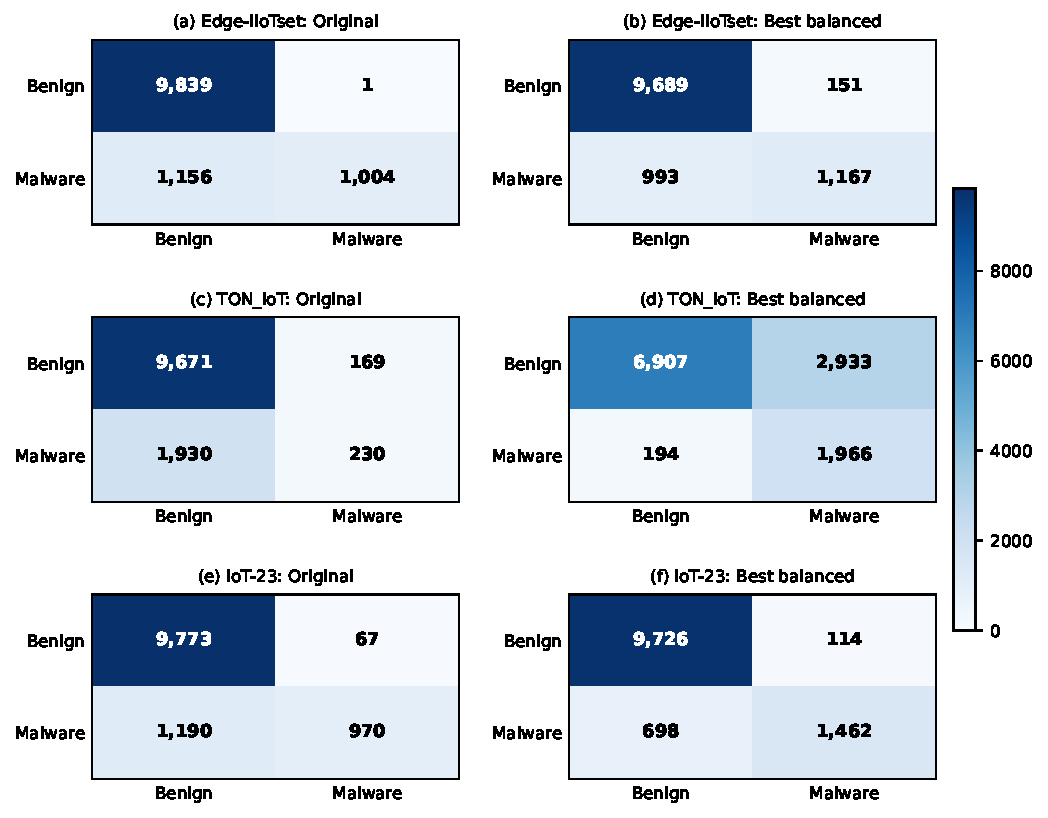
\includegraphics[width=0.84\textwidth]{figures/fig2_confusion.pdf}
\caption{LSTM confusion matrices on the fixed 12{,}000-flow test set, per dataset, in the unbalanced baseline and in the best balanced configuration (selection rule of Section~\ref{sec:method}).}
\label{fig:confusion}
\end{figure*}

Second, tree ensembles are already near-saturated under imbalance. XGBoost misses only four attacks on CICIDS2017 without any balancing, and oversampling reduces its FNs by at most 16.5\% (UNSW-NB15) while Random Forest gains at most $\approx$17\%. This is consistent with the known robustness of boosting and bagging to moderate class imbalance, and means that for ensemble-based IDSs, balancing is largely unnecessary. Fig.~\ref{fig:metrics} (F1-score heatmap) and Fig.~\ref{fig:fnfp} (FN grouped bars) visualize this across all six strategies and four models.

\begin{figure*}[!t]
\centering
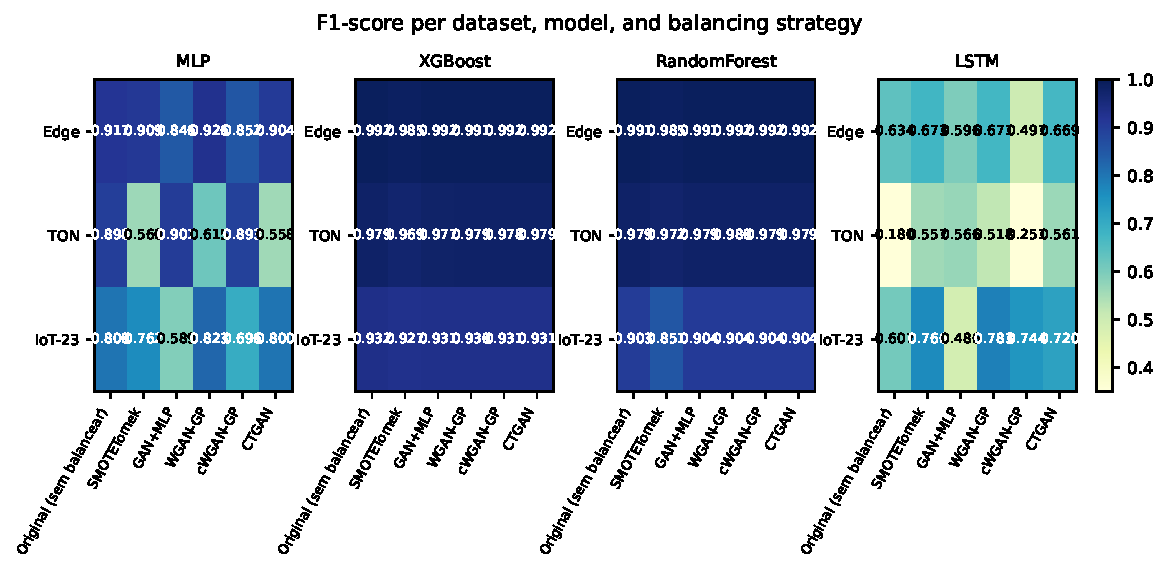
\includegraphics[width=\textwidth]{figures/fig3_metrics.pdf}
\caption{F1-score per dataset, model, and balancing strategy. The LSTM column shows the largest gap between the unbalanced baseline and the balanced scenarios.}
\label{fig:metrics}
\end{figure*}

\begin{figure*}[!t]
\centering
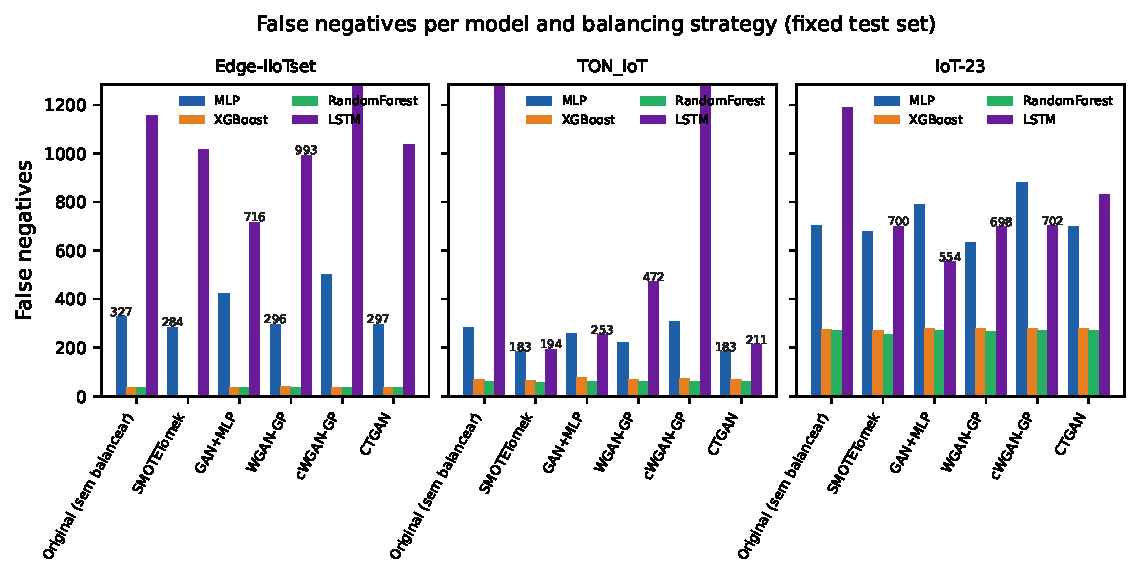
\includegraphics[width=\textwidth]{figures/fig4_fnfptp.pdf}
\caption{False negatives per model and balancing strategy on the fixed test set of each dataset.}
\label{fig:fnfp}
\end{figure*}

Third, the MLP shows no reliable benefit, and in easy problems oversampling can even regress. On CICIDS2017 the unbalanced MLP already achieves only 37 FNs---a nearly-separable problem---and the best balanced configuration (GAN) \emph{increases} that count to 60, exactly the label-noise effect expected when the synthetic samples no longer lie on the true decision boundary. On UNSW-NB15 the gain is marginal ($-4\%$) and on IoT-23 the count is statistically unchanged. The paper thus reaches a more nuanced conclusion than the ``generative oversampling is best'' headlines found in parts of the literature: the value of balancing is real but conditional on the classifier, and it is largest precisely where imbalance degrades the detector most (deep networks on hard traffic).

\subsection{The Balancing Method in Isolation}
Because for each model and dataset every scenario shares the same test set, feature set, and training split, the differences in Table~\ref{tab:cross} are attributable to the balancing strategy alone. No single strategy dominates. SMOTETomek---the classic, non-generative reference---is selected as best in six of the twelve configurations (mostly for tree ensembles and UNSW-NB15), the Wasserstein variants (WGAN-GP and cWGAN-GP) in four, and the vanilla GAN in two (the two MLP rows). CTGAN is never the unique best under the F1-guard rule, although it is consistently among the strongest for the LSTM (e.g., FNs of 230 and 207 on CICIDS2017 and UNSW-NB15 before the precision guard) and achieves the highest F1 for the UNSW-NB15 LSTM. This distributed pattern, which contradicts the notion of a single winning generator family, is precisely the kind of evidence that aggregate-metric reporting hides: reported F1 differences between scenarios are often within 0.05, while the FN/FP counts they imply can differ by an order of magnitude on the minority class.

To ensure that the winners of Table~\ref{tab:cross} are not an artifact of the 0.05 tolerance of the selection rule, we repeated the selection for tolerances of 0.00, 0.02, 0.05, and 0.10. The overall pattern is stable. For the LSTM the chosen strategy can change---UNSW-NB15 selects CTGAN under a strict rule and SMOTETomek once the tolerance reaches 0.05, and IoT-23 shifts from cWGAN-GP to WGAN-GP---but the FN reduction stays large at every tolerance: 83.1\% on CICIDS2017 at all tolerances, 75.5--81.5\% on UNSW-NB15, and 39.8--40.6\% on IoT-23. Conversely, lax tolerances can be counterproductive on easy problems: at 0.10, the UNSW-NB15 MLP would switch from the vanilla GAN (FN 404, FP 139, F1 0.87) to SMOTETomek (FN 168, FP 858, F1 0.80), trading a slightly lower FN count for a large rise in false alarms---precisely the collapse the F1-guard prevents.

\subsection{Comparison with Related Work}
Table~\ref{tab:related} positions our protocol against recent generative-oversampling NIDS studies. Direct numerical comparison is hindered by differences in datasets, features, and classifiers---precisely the problem we set out to address---but two qualitative points stand out. First, studies that report detailed minority-class metrics consistently identify recall/false negatives as the metric that generative balancing improves the most~\cite{he2023cwvaegan,yang2025cegan,babu2023mcgan}. Second, our controlled comparison shows that CTGAN-based pipelines~\cite{zha2025anids,soflaei2024dualctgan,habibi2023ctgan} are strong but not uniquely so: classic SMOTETomek matches them on several configurations, which existing single-dataset, single-classifier studies cannot reveal.

\begin{table}[!t]
\caption{Related Work on Generative Oversampling for NIDS (representative)}
\label{tab:related}
\begin{center}
\footnotesize
\setlength{\tabcolsep}{4pt}
\begin{tabular}{@{}p{0.16\columnwidth}p{0.20\columnwidth}p{0.22\columnwidth}p{0.24\columnwidth}@{}}
\toprule
\textbf{Work} & \textbf{Model} & \textbf{Datasets} & \textbf{Key contribution} \\
\midrule
\cite{habibi2023ctgan} & CTGAN & IoT-23 & CTGAN-balanced tabular modeling for IoT botnets \\
\cite{zha2025anids} & Stacked CTGAN & CICIDS-2017/18 & Drift-adaptive IDS, 5\,$\mu$s latency \\
\cite{alabsi2023ctgan} & CTGAN & CICIDS-2017 & CTGAN IDS for DDoS/DoS \\
\cite{yao2025cwgangp} & CWGAN-GP & NSL-KDD, UNSW-NB15 & Stable CWGAN-GP oversampling \\
\cite{rahman2024syngan} & SYN-GAN & UNSW-NB15, NSL-KDD, BoT-IoT & Fully-synthetic GAN training, robust IoT IDS \\
\cite{he2023cwvaegan} & CWVAEGAN\allowbreak+1D-CNN & NSL-KDD, UNSW-NB15 & VGM decomposition, high minority recall \\
\cite{park2023ainids} & GAN-based & NIDS datasets & AI-based GAN-augmented NIDS \\
\cite{soflaei2024dualctgan} & CTGAN\allowbreak+ensembles & UNSW-NB15 & 98\% binary accuracy \\
\cite{yang2025cegan} & CE-GAN & NSL-KDD, UNSW-NB15 & Composite loss, game-theoretic ensemble \\
\cite{swadi2025wcg} & WCGAN & UNSW-NB15, KDD CUP99 & Wasserstein class balancing \\
\cite{ding2024tmgggan} & TMG-GAN & CICIDS2017, UNSW-NB15 & GAN imbalanced learning \\
\textbf{Ours} & \textbf{6 strategies} & \textbf{IoT-23, UNSW-NB15, CICIDS2017} & \textbf{Controlled 6-way $\times$ 4-clf FN-focused benchmark} \\
\bottomrule
\end{tabular}
\end{center}
\end{table}

\subsection{Computational Cost}
The balancing overhead is dominated by the generative strategies: training each generator for 300 epochs was the single most expensive step of every scenario, whereas SMOTETomek (pure resampling) and the classifiers added only seconds. Table~\ref{tab:cost} reports the wall-clock time of the four generator training loops, measured on the same Google Colab GPU profile while executing the notebooks that produced the results of Table~\ref{tab:cross}. The vanilla GAN (Section~\ref{sec:method}), whose generator/discriminator loops run in interpreted Python, is by far the slowest and consumed $\approx$16--17~min per dataset ($\approx$4.5$\times$ the WGAN-GP). The Wasserstein variants converge in 3.7--4.7~min, and CTGAN in 2.4--7.5~min, scaling with the number of minority-class flows. Training all four generators still takes under 33~min per dataset, comfortably within a single Colab session.

\begin{table}[!t]
\caption{Generator Training Time per Dataset (wall-clock seconds, single GPU, 300 epochs)}
\label{tab:cost}
\begin{center}
\footnotesize
\setlength{\tabcolsep}{6pt}
\begin{tabular}{@{}lcccc@{}}
\toprule
\textbf{Dataset} & \textbf{GAN} & \textbf{WGAN-GP} & \textbf{cWGAN-GP} & \textbf{CTGAN} \\
\midrule
CICIDS2017 & 1008 & 223 & 281 & 450 \\
UNSW-NB15 & 956 & 224 & 275 & 263 \\
IoT-23 & 954 & 225 & 263 & 143 \\
\bottomrule
\end{tabular}
\end{center}
\end{table}

\subsection{Threats to Validity}
Several limitations should be acknowledged. First, all three datasets are real and public, but the IoT-23 subset used here consists of 6.05M Zeek \texttt{conn.log} flows prepared by a third-party preprocessing, which covers a large but not complete portion of the official IoT-23 captures; its features (Zeek fields) differ in nature from the CICFlowMeter features of the other two datasets, even though the pipeline is identical. Second, results are reported for a single split and seed and without hyperparameter search; the fixed protocol guarantees internal reproducibility, but we do not quantify split-to-split variance. Third, the ``best balanced configuration'' is selected post-hoc by an explicit, a-priori rule (Section~\ref{sec:method}) that guards against precision collapse, yet multiple-testing across six strategies could inflate the chance of selecting a spuriously low FN; we therefore emphasize effect \emph{patterns} across datasets (e.g., the LSTM consistently improving) rather than individual best rows. Fourth, synthetic samples were validated only implicitly, via downstream classification and PCA projections, rather than with formal fidelity tests (e.g., train-on-synthetic/test-on-real, KS statistics). Fifth, our study is restricted to binary classification (benign vs.\ malware); multiclass per-family detection and per-capture analysis of the IoT-23 records remain open. Finally, only four classifier families were considered; modern convolutional and attention-based detectors were not evaluated.

\section{Conclusion and Future Work}
\label{sec:conclusion}
We presented a strictly controlled comparison of six balancing strategies---none, SMOTETomek, vanilla GAN, WGAN-GP, cWGAN-GP, and CTGAN---for binary intrusion detection, reproduced identically on three real datasets (CICIDS2017, UNSW-NB15, and IoT-23) and four classifiers (MLP, XGBoost, Random Forest, and LSTM), with a shared workload, split, feature-selection step, and test set. The results show that the benefit of balancing is strongly classifier-dependent. The deep sequential model, which is the most degraded by imbalance (unbalanced F1 of 0.33--0.71 across datasets), is also the most improved by resampling, with false negatives reduced by 83.1\% on CICIDS2017 ($1{,}716\rightarrow290$), 81.5\% on UNSW-NB15 ($845\rightarrow156$), and 40.6\% on IoT-23 ($1{,}169\rightarrow694$). Tree ensembles, near-saturated under imbalance, gain at most marginally (0--17\%), and the MLP shows no reliable benefit, regressing on easy problems. No single balancing strategy dominates: classic SMOTETomek and Wasserstein-based generative methods alternate as best across configurations, and CTGAN is consistently strong but not uniquely so.

These nuances are invisible in accuracy- or F1-only reporting, which motivates the main methodological contribution of this work. Beyond the empirical results, we contribute an evaluation protocol whose central claim is \emph{honesty}: imbalance studies in NIDS should (i) report confusion-matrix counts---especially false negatives, the security-critical error---as first-class metrics, (ii) isolate the balancing effect from the classifier choice by keeping workload, split, feature-selection step, and test set fixed, and (iii) state a-priori a selection rule that refuses a false-negative reduction bought at the price of a collapsed F1. We deliberately do \emph{not} claim that resampling drastically reduces FNs in all settings; the evidence shows the benefit is strongly classifier- and dataset-dependent, and our protocol is explicitly designed so that these nuances are reportable rather than averaged away. Our reproducible template---code, notebooks, and datasets in a public repository---lets any reader re-run the six-strategy, four-classifier comparison on their own data and obtain the confusions we report.

Future work includes (i) extending the benchmark to multiclass per-family detection, to the full IoT-23 capture, and to Edge-IIoTset~\cite{ferrag2022edgeiiotset}; (ii) evaluating train-on-synthetic/test-on-real fidelity metrics and differential-privacy-preserving generation; (iii) combining balancing with focal loss~\cite{dina2023focal} and non-sequential deep detectors (CNNs, transformers) to test whether the LSTM-specific finding generalizes; and (iv) quantifying split-to-split variance through repeated-seed cross-validation.

\bibliographystyle{IEEEtran}
\bibliography{references}

\end{document}